\chapter{Implementation}
\label{sec:implementation}

All aspects of \Backpack{}, as described in this thesis,
have been implemented in GHC 8.2 and cabal-install 2.0.  In this
chapter, we describe some aspects of our implementation.

\section{Modifications to GHC}

Here is a brief summary of the modifications we made to
GHC in order to support \Backpack{}, with parenthesized pointers to the
affected modules in GHC's code base:

\begin{itemize}
    \item Support for the merging rules: especially the rules for
    export list merging (\verb|NameShape|, which also implements the
    code for treating an export list as a name substitution) and
    declaration merging (in \verb|TcIface|).

    \item Support for the substitution rules (\verb|RnModIface|)
    on GHC's interface representation (see Section~\ref{sec:no-symbol-tables}).

    \item Modifications to GHC's core \verb|Module| and \verb|Name| data
    types to support module and name holes.  In fact, a module hole $\hv{m}$
    is represented as a regular module identity with the special unit
    identity \verb|hole|; similarly, a name hole \nhv{m.n} is represented
    as the name $n$ from the module hole $\hv{m}$.  Internally representing
    the holes this way was expedient as it allowed us to avoid having to
    add a lot of new pattern matches to GHC, but the tradeoff is that
    we have to be careful about how we go about performing substitutions.

    \item Modification to GHC's \verb|UnitId| data type to support module
    substitutions.  We try to keep \uid{}s represented as plain
    strings as much as possible; see Section~\ref{sec:opaque-uid} for
    more details.

    \item Support for the lookup rules, which were done by modifying
    GHC's mechanism for looking up declarations from interface files
    (\verb|LoadIface|) to first substitute according to the \uid{}.
    Because declaration type lookup always goes through the interface
    lookup process, it meant we only needed to modify one place in the
    compiler to support instantiation.

    \item Support for the signature matching rules
    (\verb|TcBackpack|).

    \item Support for the dependency typing rules, which were hooked into
    the existing \verb|GhcMake| compilation driver. The implementation
    here is a little bit of a cheat: you \emph{must} use \verb|ghc --make|
    to check if dependencies are well-typed, as there is no
    one-shot compiler mode you can use to apply this check.

    \item Support for the \textsf{inherits} and \textsf{exposes} procedures
    (\verb|Packages|).

    \item Support for the \verb|bkp| file format: we needed
    a new frontend driver for GHC (\verb|DriverBkp|), abstract syntax (\verb|BkpSyn|)
    and some modest lexer and parser extensions (\verb|Lexer| and \verb|Parser|).
    Arguably, these bits aren't part of the implementation ``proper'', since
    they're only used for testing.

    \item Support for typechecking signature files (\verb|TcRnDriver|)
    and signature merging (\verb|HscMain|).  Here, we were a bit lucky:
    GHC's existing \verb|hs-boot| files closely resemble \verb|hsig|
    files, and we were able to repurpose a lot of the existing code in
    our implementation.

    \item Miscellaneous modifications to GHC's existing behavior,
    such as modifying GHC's constraint solver to not eagerly fail when
    simplifying givens (Section~\ref{sec:substitutability}).
\end{itemize}
%
In our primary \Backpack{} patch (not counting subsequent bugfix
patches, as well as some preliminary support for signatures that we had
committed previously), we modified 40 files in the compiler (out of 513
source files in the \verb|compiler| directory), adding 4375 lines and
deleting 588 lines.  In this respect, we think that our \Backpack{}
patch is quite well-contained: by in large, we were able to implement
\Backpack{} without touching the renamer or typechecker: \Backpack{}
interposed on the interface file loading layer to transparently
provide a type environment that looked exactly like the old type
environment (except with more elaborate \uid{}s).  We did have to
modify some core data types in GHC, but as most of the compiler
treated these abstractly, this did not cause any large ripple effects.

\subsection{No symbol tables}
\label{sec:no-symbol-tables}

One aspect of GHC's design which is worth calling out is its lack
of symbol tables.
Compilers usually have one or more data structures known as
\emph{symbol tables}, which are mappings from symbols to information
about the symbol: abstractly, the symbol table is represented by
the \emph{context} in which typechecking takes place.
In contrast, GHC avoids symbol tables:  instead, a
symbol \emph{contains} all information about itself, forming an
immutable \emph{cyclic data structure} of all symbols
known to GHC\@.  For example, here are
some data types for the graph representation from GHC (simplified
and abbreviated):

\begin{lstlisting}
    data Type  = TyConApp TyCon [Type]  | ...
    data TyCon = SynonymTyCon Name Type | ...
    data ModDetails = ModDetails [TyCon] ...
\end{lstlisting}
%
A type may be an application of a type constructor to some arguments, in which
case it contains a type constructor \verb|TyCon|.  A type constructor
can be a type synonym, in which case it contains the type it expands
to.  A module \verb|ModDetails| consists of a list of type constructors
and other entities that are defined in it.  The ``graph'' is the graph of
heap objects which represent these data types.

This graph is very convenient to work with in a purely functional
language like Haskell, since queries can be answered by a direct field
access rather than a lookup in a symbol table.  For example, type
equality can be defined as a pure function \verb|Type -> Type -> Bool|
even in the presence of type synonyms, since the \verb|SynonymTyCon|
always carries along the expanded version of the synonym to compare
against.

On disk, GHC doesn't store an infinite type; instead, its
interface representation closely resembles the semantic objects
we described in Section~\ref{sec:semantic-objects}:

\begin{lstlisting}
    data IfaceType = IfaceTyConApp Name [IfaceType] | ...
    data IfaceDecl = IfaceSynonym OccName IfaceType | ...
    data ModIface = ModIface [IfaceDecl] ...
\end{lstlisting}

\noindent
Unlike the graph representation, the type constructor application
doesn't embed the definition of the type constructor---instead,
it records only a \verb|Name| reference to the constructor. To find out
more information about the type constructor, you would have to lookup
the \verb|IfaceDecl| from the appropriate symbol table; e.g., a module
local declaration would be found in the \verb|IfaceDecl| list in
\verb|ModIface|.

GHC uses a technique called ``tying the knot''
to construct the graph representation from the interface
representation: any time we encounter a \verb|Name|, GHC instead
allocates a thunk to lookup the appropriate declaration later,
once all of the entities have been added to the environment.

\paragraph{Consequences for \Backpack{}}
In Section~\ref{sec:overview-compiler}, we informally described
types as graphs, with original names pointing to the corresponding
declaration.  In fact, this is an accurate representation of how
these operations are implemented in GHC\@!

One downside of the immutable graph representation is that it is
difficult to modify after the fact: in general, the only way to update
it is to rebuild the graph from scratch.  Modifications of this kind
frequently occur in \Backpack{}: for example, applying a name
substitution will change how the graph is wired.

To handle this, our implementation does most operations in two
phases:

\begin{itemize}
    \item We first perform any operations which would
    mutate the graph on the \emph{interface representation}.
    These operations includes both module and name substitutions, as well
    as signature merging.
    \item Then, we generate the \emph{graph representation} from
    the resulting interface representation, and then perform any
    operations which require consulting the context.  These
    operations include subtyping, which test equality on types
    and require the context.
\end{itemize}
%
Our typechecking rules are staged so that once we have generated the
graph representation, we don't need to regenerate it in the future.

\section{Modifications to Cabal}

Before discussing how \Backpack{} was integrated with Haskell's
package manager Cabal, we first need to give a more detailed description
of how Cabal is structured architecturally.

What users colloquially refer to as ``Cabal'' actually refers to two
distinct pieces of software: Cabal the build system, and cabal-install
the package manager.  Cabal is solely concerned with the problem of building
a single \emph{package} (which may contain multiple components), while
cabal-install manages the problem if installing multiple packages.  The
command line interface of a Setup script intermediates between
Cabal and cabal-install:

In principle, the only major implementation piece necessary for \Backpack{}
in Cabal is mixin linking.  But it turned out it was necessary to
make some architectural changes to Cabal

Our implementation of \Backpack{} in

\section{Opaque unit identifiers}
\label{sec:opaque-uid}

\Uid{}s are abstract syntax trees which are passed around throughout
the compiler.  The downside is that instantiated \uid{}s
can be quite large (in part because \cid{}s allocated by the
package manager can be quite large, as they must record information
about how dependency resolution was performed for the library),
wasting memory in the compiler.

Fortunately, in some cases, the structure of a \uid{} is not necessary;
for example, when a unit identifier has no module holes, it is
invariant under substitution.  A useful optimization in this case
is to represent the structure opaquely with a \emph{definite unit
identifiers}.

GHC and Cabal implement this optimization, changing the
abstract structure of a \uid{} to look like this:

\[
\begin{array}{rcll}
  \mathbb{P} &&& \text{Definite \uid{}} \\
  \UP &::=& \icid{\Up}{S} & \text{\Uid} \\
      & | & \mathbb{P} \\
\end{array}
\]

\noindent
Notice that definite \uid{}s occur recursively: the intent is that a
definite \uid{} be allocated for a library when it is fully instantiated
and compiled.  Thus, a definite \uid{} always corresponds to a \uid{}
whose module substitution refers all to definite \uid{}s (since those
libraries had to be compiled first, before this one could be compiled!)
When compiling a fully instantiated library, the only \uid{}s which the
compiler needs to interact with are definite \uid{}s, meaning that we
only have to pay the cost of a full \uid{} when typechecking uninstantiated
libraries.

Definite \uid{}s are purely an implementation mechanism; if a definite
\uid{} and a normal \uid{} are compared, the comparison must be done
up to unfoldings of the definite \uid{}, as seen below (definite \uid{}s
highlighted in blue):

\begin{figure}[H]
\center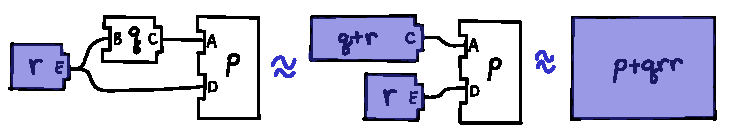
\includegraphics{figures/unit-identifier-improvement.pdf}
\end{figure}
